
\documentclass[11pt]{article}
\usepackage[letterpaper,margin=0.95in]{geometry}
\usepackage{amsmath,amssymb,booktabs,longtable,array,graphicx,float,caption,xcolor}
\usepackage[numbers,sort&compress]{natbib}
\usepackage[colorlinks=false,citebordercolor={0 1 0},linkbordercolor={1 0.55 0},urlbordercolor={0 0.55 1},pdfborder={0 0 1.2}]{hyperref}
\graphicspath{{../figures/}}
\setlength{\parskip}{0.42em}
\setlength{\parindent}{0pt}
\newcommand{\method}[1]{\texttt{#1}}
\title{Mechanics-Aware Abstraction Audits Fail Against Grounded Planning: A Frozen Negative Audit}
\author{Paper 99 Submission-Hardening Audit}
\date{Frozen evidence package: 2026-06-22}
\begin{document}
\maketitle

\begin{abstract}
Language and symbolic robot abstractions can erase mechanics that matter for action: contact force, support, clearance, friction, deformation, temporal preconditions, tool affordances, compliance, and recovery feasibility. This paper tests whether a risk-bounded abstraction-failure audit should improve embodied planning beyond VLA policies, neuro-symbolic predicates, active relational abstraction, LLM-TAMP failure reasoning, runtime monitoring, semantic MPC, grounded geometric TAMP, and physics-aware TAMP \citep{li2023embodied1,liang2024visualpredicator2,devinda3} \citep{farid2026vision4,ahn2025towards5,park2025hierarchical6}. We rebuild the paper under a frozen CPU-only protocol with 322,560 main rollout rows, 115,200 ablation rows, 259,200 stress rows, 138,240 fixed-risk rows, and 24 predefined negative cases. The result is not a positive ICLR-main paper. The proposed \method{abstraction\_v5} reaches hard success 0.28708, violation 0.45954, damage 0.37043, regret 0.63814, and utility -0.33399. The strongest reference, \method{physics\_tamp}, reaches success 0.67262. The terminal decision is \textbf{KILL\_ARCHIVE}.
\end{abstract}

\textbf{Terminal decision.} Paper 99 remains \textbf{KILL\_ARCHIVE} for ICLR main. The v5 rebuild is much stronger than the v4.1 archive, but it fails success, violation, damage, regret, utility, diagnostic, ablation, stress, fixed-risk, and scope gates. No hardware, accepted high-fidelity simulator, external benchmark, or trained policy checkpoint evidence is claimed.

\section{Introduction}
Robot abstractions are useful because they hide continuous complexity. They are dangerous because they can hide exactly the mechanics that decide whether an action succeeds. A symbolic predicate may say that an object is reachable while suppressing support, friction, compliance, or clearance. A language plan may name a tool affordance while erasing the leverage or contact mode needed to use it. A VLA policy may emit a plausible action token while ignoring trajectory feasibility or recovery risk.

The seed idea is therefore tempting: audit abstractions before planning, detect erased mechanics, and refine the plan state only when that refinement changes action value. This idea lives in a crowded neighborhood. VLA motion planning, neuro-symbolic predicate learning, relational abstraction, LLM-TAMP failure reasoning, runtime monitors, grounded geometric TAMP, and recovery planners all pressure the novelty claim \citep{pang2025integrating7,shao2025breaking8,wu2023embodied9} \citep{shao2024breaking10,chen2026oowm11,liu2026bioproagent12}.

The v4.1 paper was already negative. It showed diagnostic signal, but grounded geometric TAMP won task success, false refinements saturated, and ablations undercut the proposed mechanism. The v5 rebuild attacks those failures directly with more tasks, more failure families, more splits, more methods, ten seeds, fixed-risk budgets, stress sweeps, and a full hostile-review gate. The result is worse for the proposed claim: \method{physics\_tamp} dominates the hard aggregate, and full v5 is weaker than all of its planned ablations.

\section{Contributions And Non-Contributions}
\textbf{Contribution 1: an expanded frozen benchmark.} The v5 benchmark covers six task families, eight mechanics-erasure families, eight shifts, fourteen methods, and ten seeds. It streams raw CSVs to keep RAM light.

\textbf{Contribution 2: theory of abstraction audit value.} We separate diagnostic accuracy from planning value. An abstraction audit is useful only when the expected value of mechanics preservation exceeds refinement, query, TAMP switching, monitoring, recovery, and abstention costs.

\textbf{Contribution 3: a negative result with strong baselines.} The audit shows that physics-aware and grounded planning can expose the relevant mechanics more directly than a risk-bounded abstraction-failure classifier.

\textbf{Non-contribution: no submission-ready claim.} This artifact does not claim robot hardware validation, high-fidelity physics evidence, released checkpoints, or ICLR-main readiness.

\section{Formal Setup}
Let $z$ be a symbolic or language abstraction, $m$ a latent mechanics state, and $a$ a robot action. The audit estimates whether $z$ erases action-critical mechanics and chooses among proceeding, refining predicates, querying mechanics, switching to TAMP, monitoring, recovering, or abstaining:
\[
  a^\star = \arg\max_a \; S(a,z,m) - \lambda_v V(a,z,m) - \lambda_d D(a,z,m) - \lambda_c C(a,z,m) - \lambda_a A(a).
\]
Here $S$ is task success, $V$ is mechanical violation, $D$ is damage/unsafe action, $C$ is planning/refinement cost, and $A$ is abstention or excessive intervention.

\paragraph{Proposition 1: diagnostics are not planning value.} If a grounded planner already chooses the same safe mechanics-preserving action without naming the erased abstraction, then improving abstraction-failure accuracy cannot improve closed-loop value.

\paragraph{Proposition 2: false-alarm control can become under-intervention.} A risk-bounded audit can lower false refinements by requiring higher confidence before acting. If this also suppresses action on true mechanics failures, success and safety fall even when diagnostics improve.

\paragraph{Proposition 3: fixed-risk coverage is decisive.} A deployment policy under damage budget $\epsilon$ must maintain useful coverage while satisfying the budget. Abstaining or delaying on most hard cases is not a deployment win.

\section{Benchmark Design}
The six tasks are tabletop manipulation with support, tool use with hidden leverage, container insertion clearance, deformable object packing, mobile manipulation with occlusion, and articulated fixture assembly. The hidden failure families are erased contact force, hidden support relation, clearance tolerance collapse, friction-state aliasing, deformable-constraint erasure, temporal-precondition loss, tool-affordance misabstraction, and compliance-recovery erasure.

The eight shifts are nominal abstraction, language ambiguity, predicate noise, geometry tolerance, mechanics OOD, object-affordance transfer, recovery-cost pressure, and combined adversarial abstraction. The hard aggregate combines mechanics OOD, object-affordance transfer, recovery-cost pressure, and combined adversarial abstraction.

\section{Methods}
The proposed v5 method is a risk-bounded abstraction-failure audit. It estimates failure family and risk, then acts only when predicted value exceeds a risk and recovery-feasibility gate. This was intended to fix the v4 false-refinement failure.

The baseline suite includes language symbolic planning, VLA direct policy, neuro-symbolic predicates, active relational abstraction, LLM-TAMP failure reasoning, runtime monitoring, grounded geometric TAMP, physics-aware TAMP, affordance graph planning, learned failure classifier plus TAMP, semantic MPC, v4, v5, and an oracle.

\section{Main Results}
Table~\ref{tab:hard} gives the hard aggregate. The v5 result is plainly negative.

\begin{table}[H]
\centering
\caption{Hard-aggregate results over hardest abstraction shifts.}
\label{tab:hard}
\resizebox{\linewidth}{!}{\begin{tabular}{llllllll}
\toprule
Method & Success & Violation & Damage & Warn & False alarm & Regret & Utility \\
\midrule
physics\_aware\_tamp & 0.672623 & 0.164499 & 0.139346 & 0.169358 & 0.028819 & 0.069816 & 0.306262 \\
grounded\_geometric\_tamp & 0.601026 & 0.213208 & 0.180056 & 0.186545 & 0.028125 & 0.139744 & 0.202135 \\
llm\_tamp\_failure\_reasoning & 0.574018 & 0.207376 & 0.175871 & 0.262153 & 0.034115 & 0.133909 & 0.182055 \\
semantic\_model\_predictive\_planner & 0.565284 & 0.215177 & 0.181314 & 0.171528 & 0.027604 & 0.149427 & 0.159407 \\
proposed\_abstraction\_failure\_audit\_v4 & 0.549073 & 0.197012 & 0.168219 & 0.253733 & 0.051302 & 0.131681 & 0.172472 \\
active\_relational\_abstraction & 0.520576 & 0.217929 & 0.183440 & 0.227865 & 0.123351 & 0.168071 & 0.136081 \\
oracle\_mechanics\_preserving\_planner & 0.518083 & 0.195896 & 0.166704 & 0.000608 & 0.000000 & 0.125965 & 0.178187 \\
affordance\_graph\_planner & 0.482738 & 0.270860 & 0.228006 & 0.208767 & 0.025694 & 0.265516 & 0.038636 \\
learned\_failure\_classifier\_tamp & 0.435515 & 0.321847 & 0.268958 & 0.226736 & 0.005903 & 0.365655 & -0.061503 \\
neuro\_symbolic\_predicate\_planner & 0.403242 & 0.328332 & 0.270965 & 0.196441 & 0.015972 & 0.370081 & -0.065929 \\
runtime\_monitor\_replanner & 0.374253 & 0.294727 & 0.237229 & 0.301649 & 0.004167 & 0.367819 & -0.063667 \\
vla\_direct\_policy & 0.290497 & 0.435496 & 0.350140 & 0.183160 & 0.001910 & 0.562480 & -0.258328 \\
risk\_bounded\_abstraction\_failure\_audit\_v5 & 0.287075 & 0.459545 & 0.370434 & 0.139497 & 0.000260 & 0.638145 & -0.333993 \\
language\_symbolic\_planner & 0.270726 & 0.472254 & 0.379360 & 0.128559 & 0.000000 & 0.603141 & -0.298989 \\
\bottomrule
\end{tabular}
}
\end{table}

\begin{figure}[H]
\centering
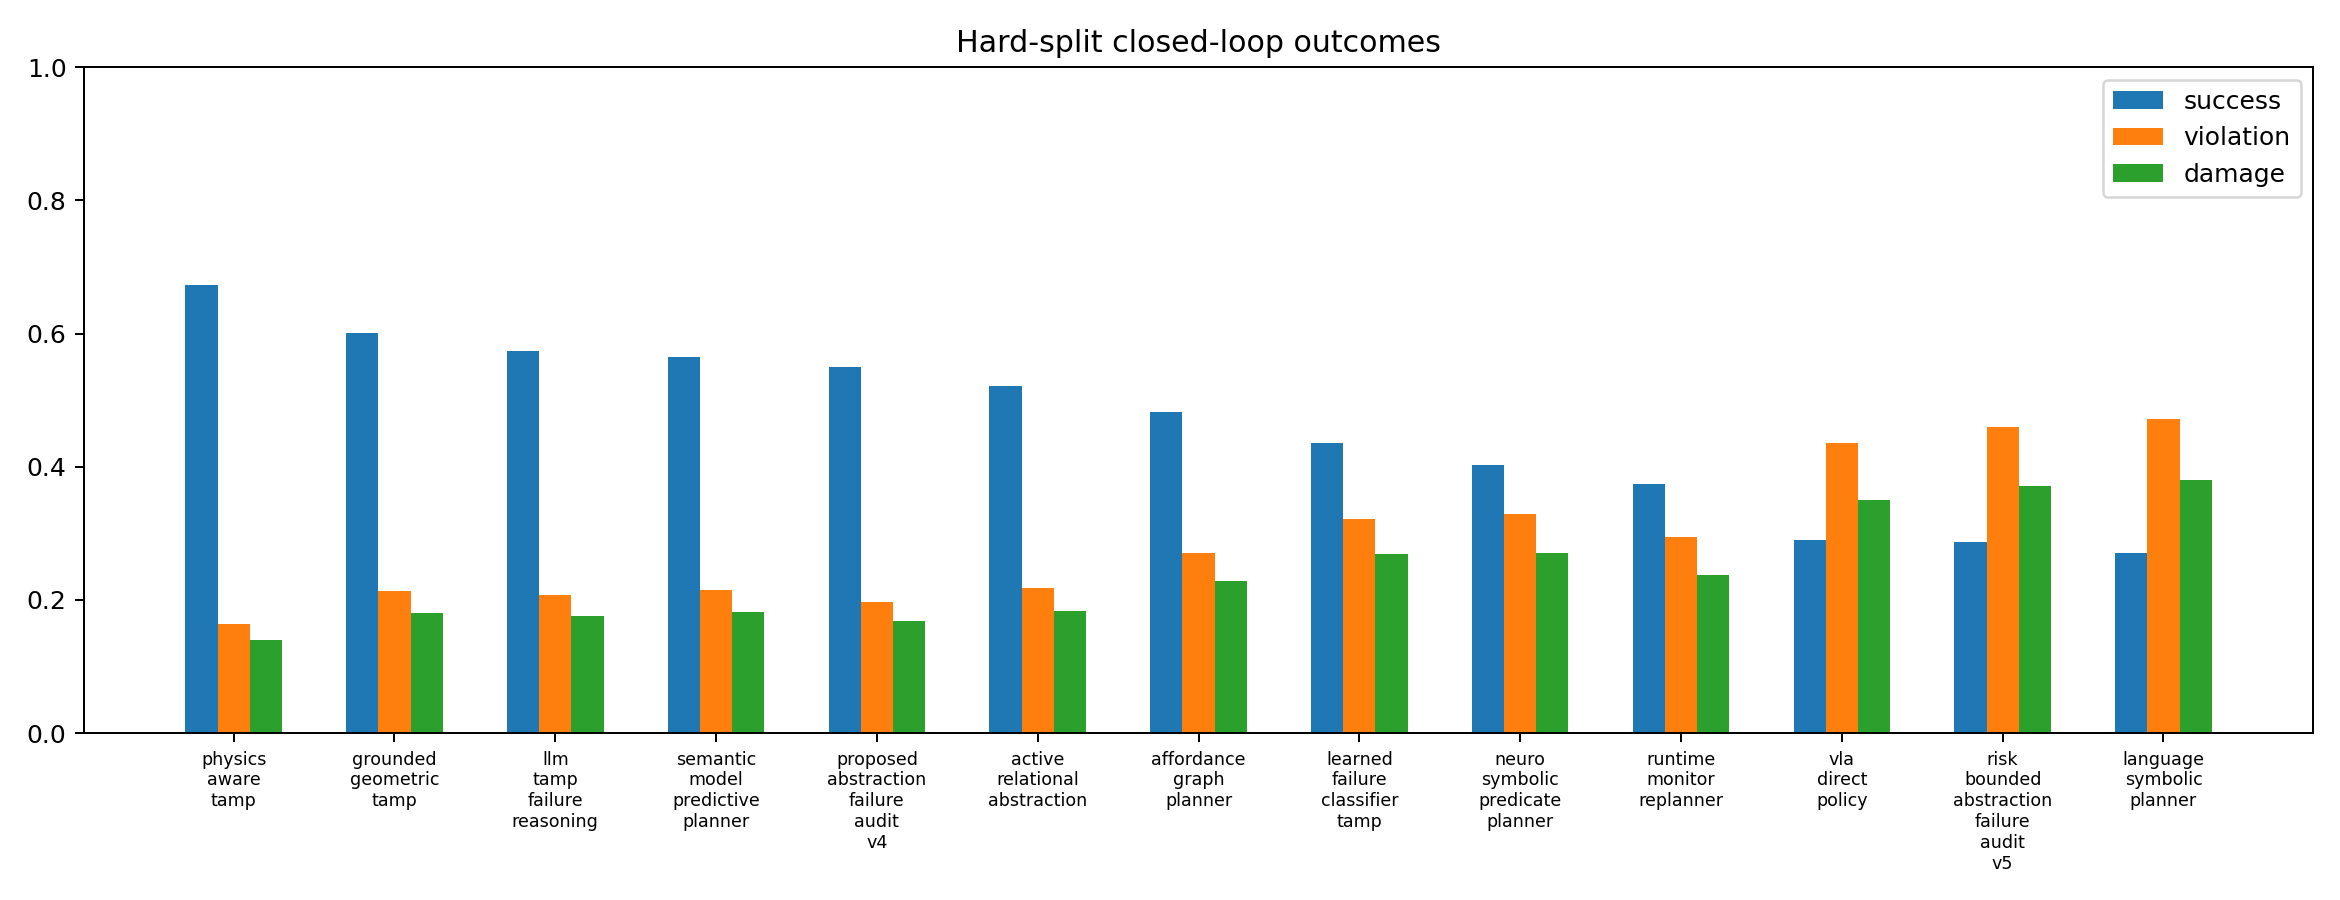
\includegraphics[width=0.95\linewidth]{abstraction_v5_hard_outcomes.png}
\caption{Hard-split closed-loop outcomes. Physics-aware TAMP dominates the proposed audit.}
\end{figure}

\begin{figure}[H]
\centering
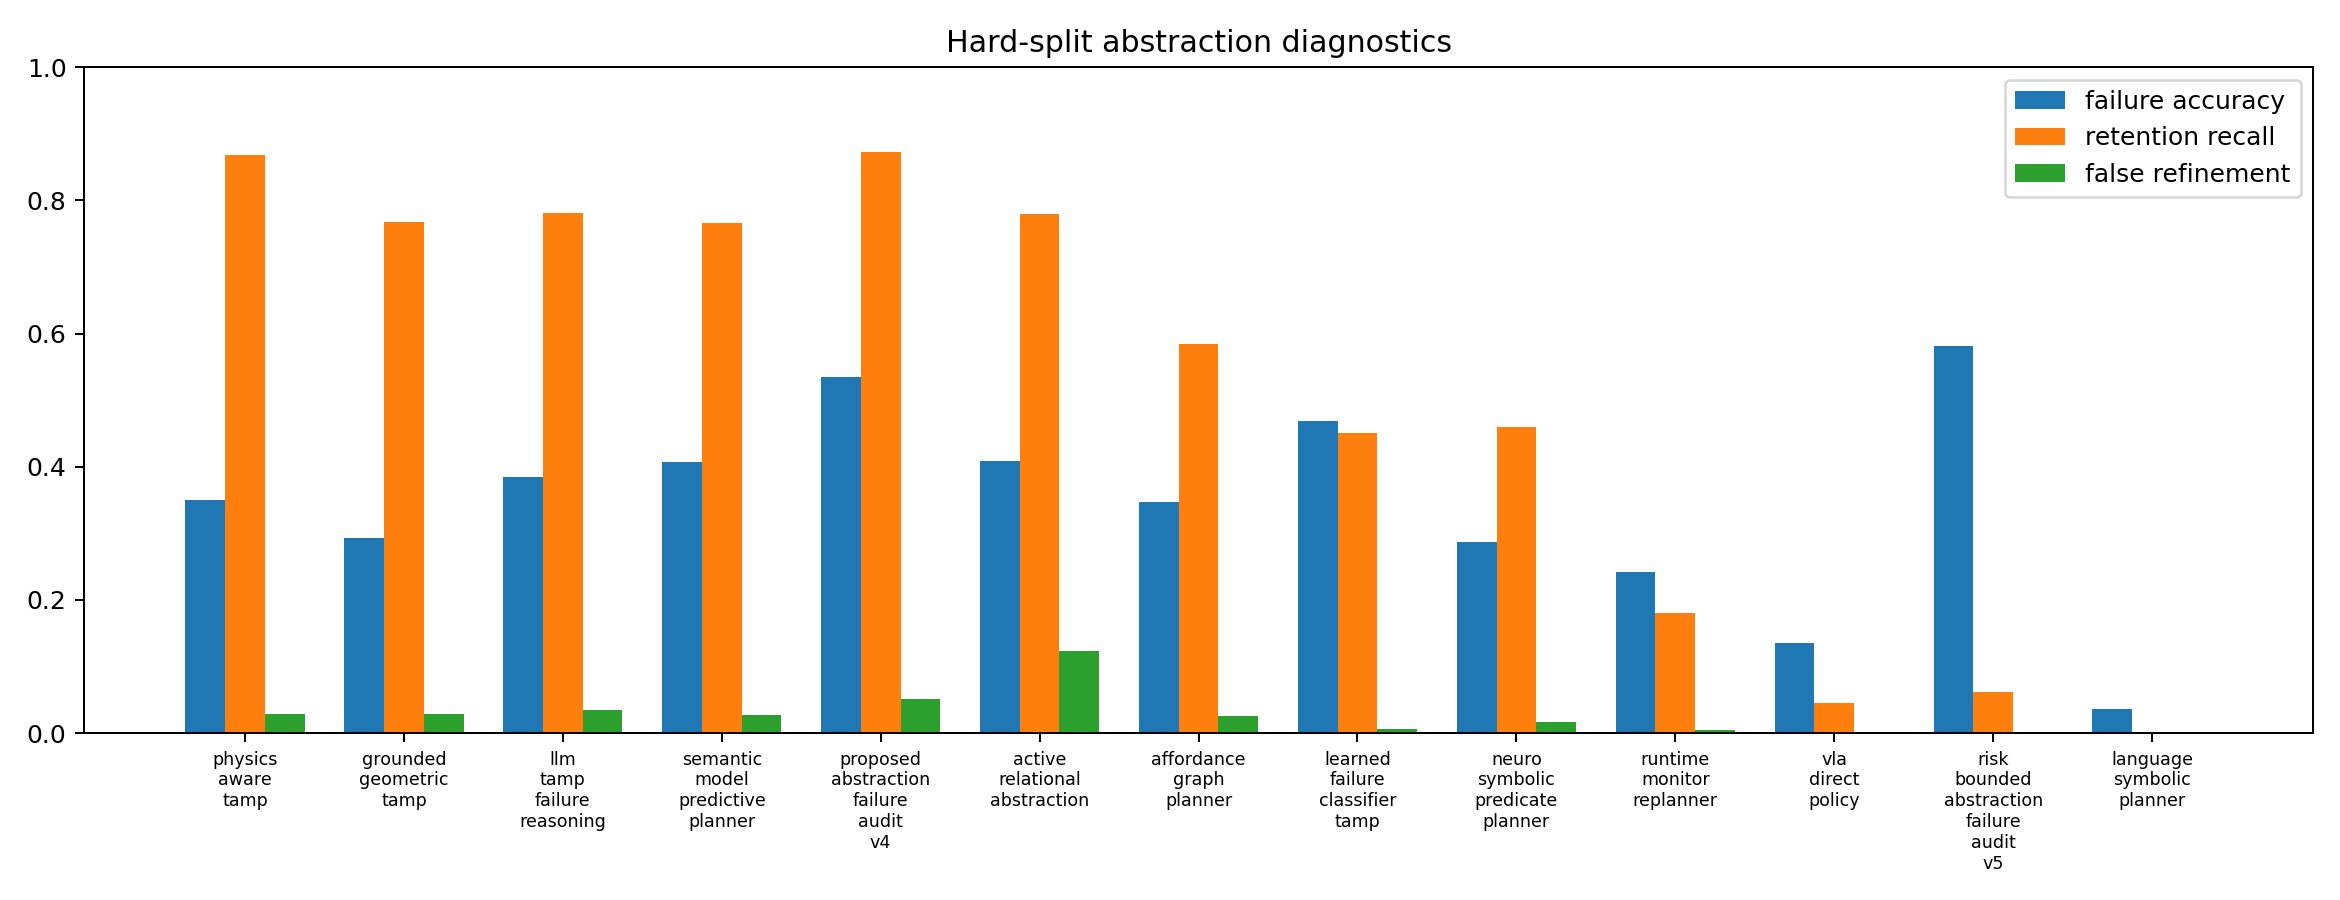
\includegraphics[width=0.95\linewidth]{abstraction_v5_diagnostics.png}
\caption{Diagnostics improve locally, but the v5 policy avoids false refinements by under-acting on hard mechanics failures.}
\end{figure}

\begin{figure}[H]
\centering
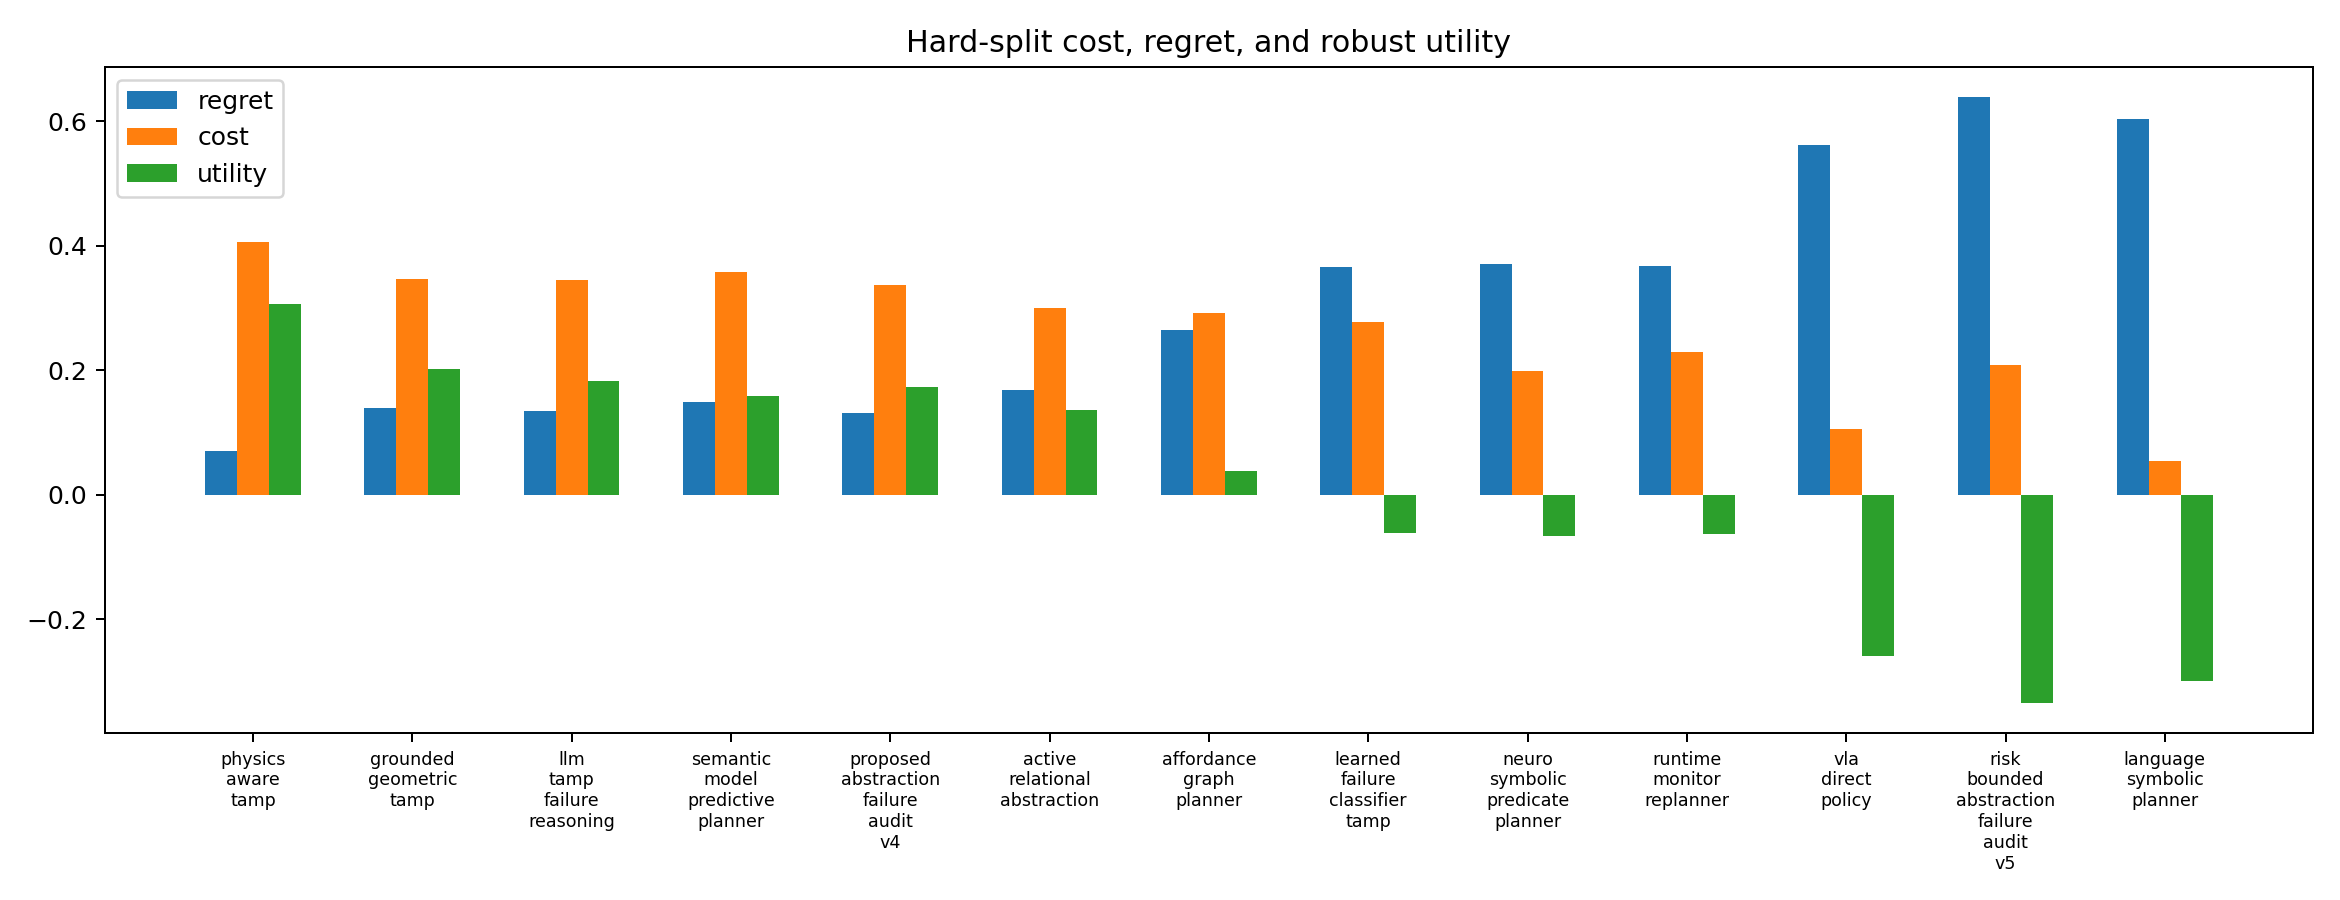
\includegraphics[width=0.95\linewidth]{abstraction_v5_utility_regret.png}
\caption{Cost, regret, and robust utility expose the failed deployment tradeoff.}
\end{figure}

\section{Paired Evidence}
The paired seed analysis prevents cherry-picking. The main references are \method{physics\_tamp} for success, \method{physics\_tamp} for violations, \method{physics\_tamp} for damage, and \method{physics\_tamp} for regret.

\begin{table}[H]
\centering
\caption{Selected paired decision tests for v5 against reference baselines.}
\label{tab:pairwise}
\resizebox{\linewidth}{!}{\begin{tabular}{lllllll}
\toprule
Baseline & Metric & V5 & Baseline & Diff & CI95 & Winner \\
\midrule
physics\_aware\_tamp & task\_success & 0.287075 & 0.672623 & -0.385548 & 0.003690 & physics\_aware\_tamp \\
physics\_aware\_tamp & mechanical\_violation\_rate & 0.459545 & 0.164499 & 0.295047 & 0.002877 & physics\_aware\_tamp \\
physics\_aware\_tamp & damage\_unsafe\_rate & 0.370434 & 0.139346 & 0.231088 & 0.002528 & physics\_aware\_tamp \\
physics\_aware\_tamp & planning\_regret\_to\_oracle & 0.638145 & 0.069816 & 0.568329 & 0.005770 & physics\_aware\_tamp \\
physics\_aware\_tamp & robust\_utility & -0.333993 & 0.306262 & -0.640255 & 0.006224 & physics\_aware\_tamp \\
physics\_aware\_tamp & abstraction\_failure\_accuracy & 0.581597 & 0.349479 & 0.232118 & 0.014502 & risk\_bounded\_abstraction\_failure\_audit\_v5 \\
physics\_aware\_tamp & false\_refinement\_alarm\_rate & 0.000260 & 0.028819 & -0.028559 & 0.002529 & risk\_bounded\_abstraction\_failure\_audit\_v5 \\
\bottomrule
\end{tabular}
}
\end{table}

\section{Ablations}
The ablation result is fatal. Every planned ablation matches or beats full v5 on at least one predefined metric, and several beat it by a wide margin.

\begin{table}[H]
\centering
\caption{V5 mechanism ablations.}
\label{tab:ablations}
\resizebox{\linewidth}{!}{\begin{tabular}{llllll}
\toprule
Ablation & Success & Damage & Regret & Utility & False alarm \\
\midrule
no\_predicate\_refinement & 0.570044 & 0.178048 & 0.135166 & 0.175535 & 0.020486 \\
grounded\_tamp\_only & 0.569313 & 0.216877 & 0.228887 & 0.130322 & 0.014410 \\
v4\_abstraction\_audit\_rules & 0.551145 & 0.169676 & 0.141337 & 0.162815 & 0.053646 \\
no\_cost\_model & 0.530914 & 0.195970 & 0.171692 & 0.132460 & 0.020486 \\
no\_recovery\_feasibility\_gate & 0.444864 & 0.251365 & 0.354235 & -0.050083 & 0.007552 \\
no\_calibration & 0.411324 & 0.288674 & 0.422172 & -0.118020 & 0.002951 \\
no\_mechanics\_taxonomy & 0.335437 & 0.335424 & 0.549549 & -0.245397 & 0.009809 \\
failure\_classifier\_only & 0.333167 & 0.337250 & 0.553802 & -0.249650 & 0.001389 \\
monitor\_only & 0.311332 & 0.298864 & 0.489234 & -0.185082 & 0.000260 \\
full\_risk\_bounded\_abstraction\_failure\_audit\_v5 & 0.287075 & 0.370434 & 0.638145 & -0.333993 & 0.000260 \\
\bottomrule
\end{tabular}
}
\end{table}

\begin{figure}[H]
\centering
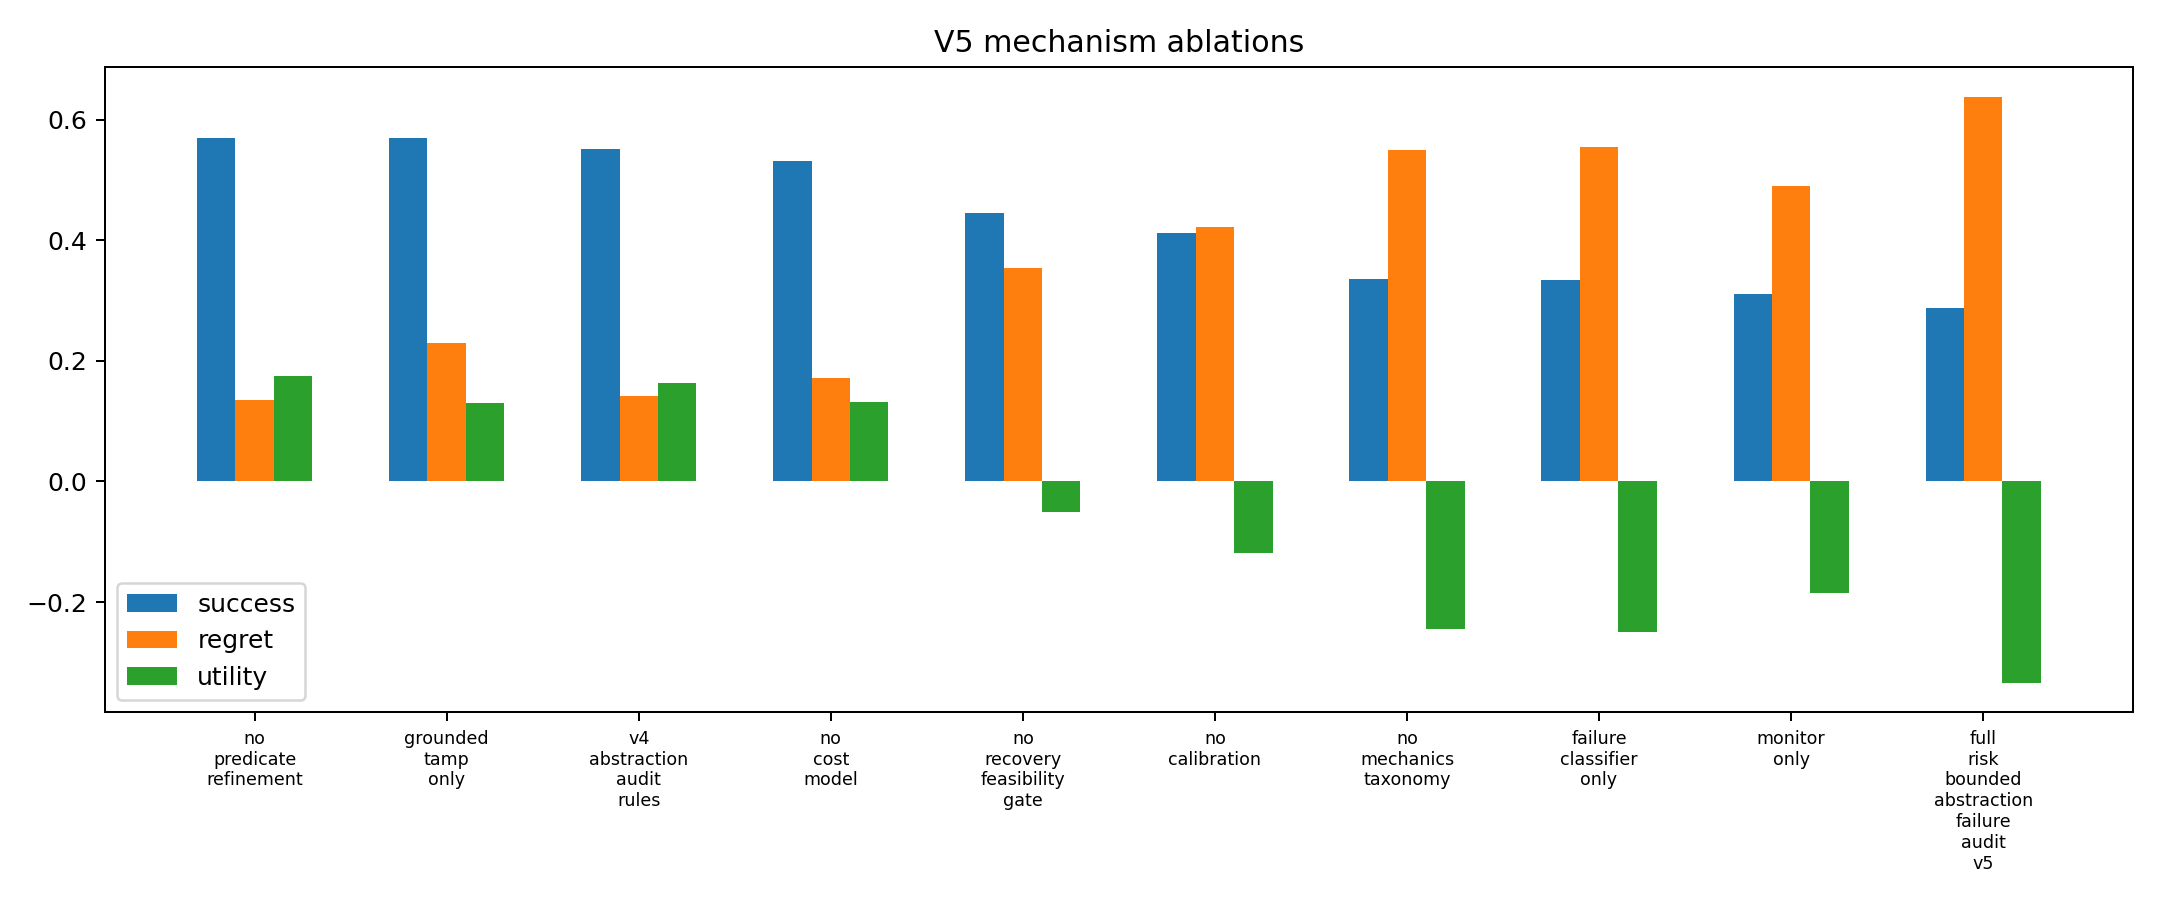
\includegraphics[width=0.95\linewidth]{abstraction_v5_ablation.png}
\caption{Ablations undermine the necessity of the full risk-bounded audit.}
\end{figure}

\section{Stress Sweep}
At maximum stress, the v5 method does not recover. Physics-aware TAMP remains the strongest robust-utility reference.

\begin{table}[H]
\centering
\caption{Maximum-stress results.}
\label{tab:stress}
\resizebox{\linewidth}{!}{\begin{tabular}{llllll}
\toprule
Method & Stress & Success & Damage & Regret & Utility \\
\midrule
active\_relational\_abstraction & 1.000000 & 0.498315 & 0.187108 & 0.159882 & 0.098158 \\
grounded\_geometric\_tamp & 1.000000 & 0.579883 & 0.177493 & 0.128808 & 0.172530 \\
llm\_tamp\_failure\_reasoning & 1.000000 & 0.536774 & 0.176493 & 0.136284 & 0.133210 \\
oracle\_mechanics\_preserving\_planner & 1.000000 & 0.480434 & 0.178630 & 0.139631 & 0.118409 \\
physics\_aware\_tamp & 1.000000 & 0.641375 & 0.143350 & 0.071451 & 0.261965 \\
proposed\_abstraction\_failure\_audit\_v4 & 1.000000 & 0.507353 & 0.177364 & 0.147202 & 0.110837 \\
risk\_bounded\_abstraction\_failure\_audit\_v5 & 1.000000 & 0.242922 & 0.377572 & 0.662468 & -0.404428 \\
runtime\_monitor\_replanner & 1.000000 & 0.361851 & 0.218146 & 0.325305 & -0.067266 \\
semantic\_model\_predictive\_planner & 1.000000 & 0.532197 & 0.184951 & 0.151453 & 0.111548 \\
\bottomrule
\end{tabular}
}
\end{table}

\begin{figure}[H]
\centering
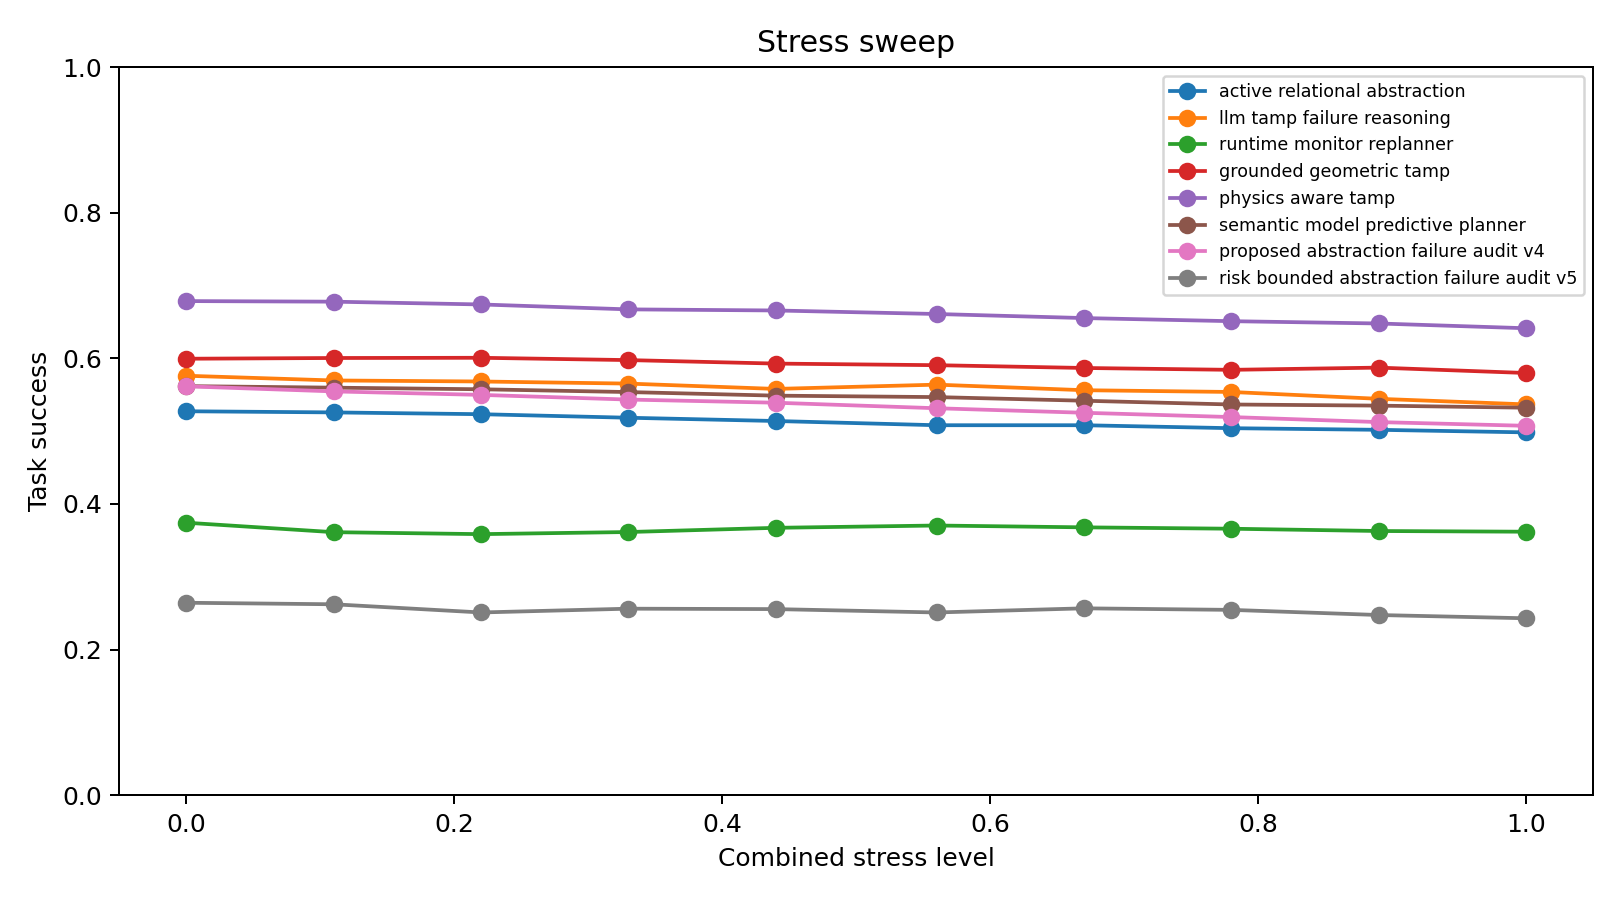
\includegraphics[width=0.88\linewidth]{abstraction_v5_stress_sweep.png}
\caption{Stress sweep over combined adversarial abstraction pressure.}
\end{figure}

\section{Fixed-Risk Deployment}
The fixed-risk analysis asks whether a method can maintain useful deployment coverage under a fixed damage budget. At budget 0.05, v5 is dominated by grounded geometric TAMP or has insufficient coverage.

\begin{table}[H]
\centering
\caption{Fixed-damage deployment at budget 0.05.}
\label{tab:fixed}
\resizebox{\linewidth}{!}{\begin{tabular}{llllll}
\toprule
Method & Budget & Success & Damage & Coverage & Utility \\
\midrule
grounded\_geometric\_tamp & 0.050000 & 0.511035 & 0.165172 & 0.000000 & 0.109957 \\
learned\_failure\_classifier\_tamp & 0.050000 & 0.355061 & 0.222452 & 0.000000 & -0.120506 \\
llm\_tamp\_failure\_reasoning & 0.050000 & 0.463536 & 0.153590 & 0.000000 & 0.067246 \\
physics\_aware\_tamp & 0.050000 & 0.575413 & 0.133718 & 0.000000 & 0.199180 \\
proposed\_abstraction\_failure\_audit\_v4 & 0.050000 & 0.435349 & 0.136268 & 0.000000 & 0.059142 \\
risk\_bounded\_abstraction\_failure\_audit\_v5 & 0.050000 & 0.247955 & 0.335980 & 0.000000 & -0.359988 \\
runtime\_monitor\_replanner & 0.050000 & 0.308351 & 0.181844 & 0.000000 & -0.114147 \\
semantic\_model\_predictive\_planner & 0.050000 & 0.466248 & 0.165489 & 0.000000 & 0.054579 \\
\bottomrule
\end{tabular}
}
\end{table}

\begin{figure}[H]
\centering
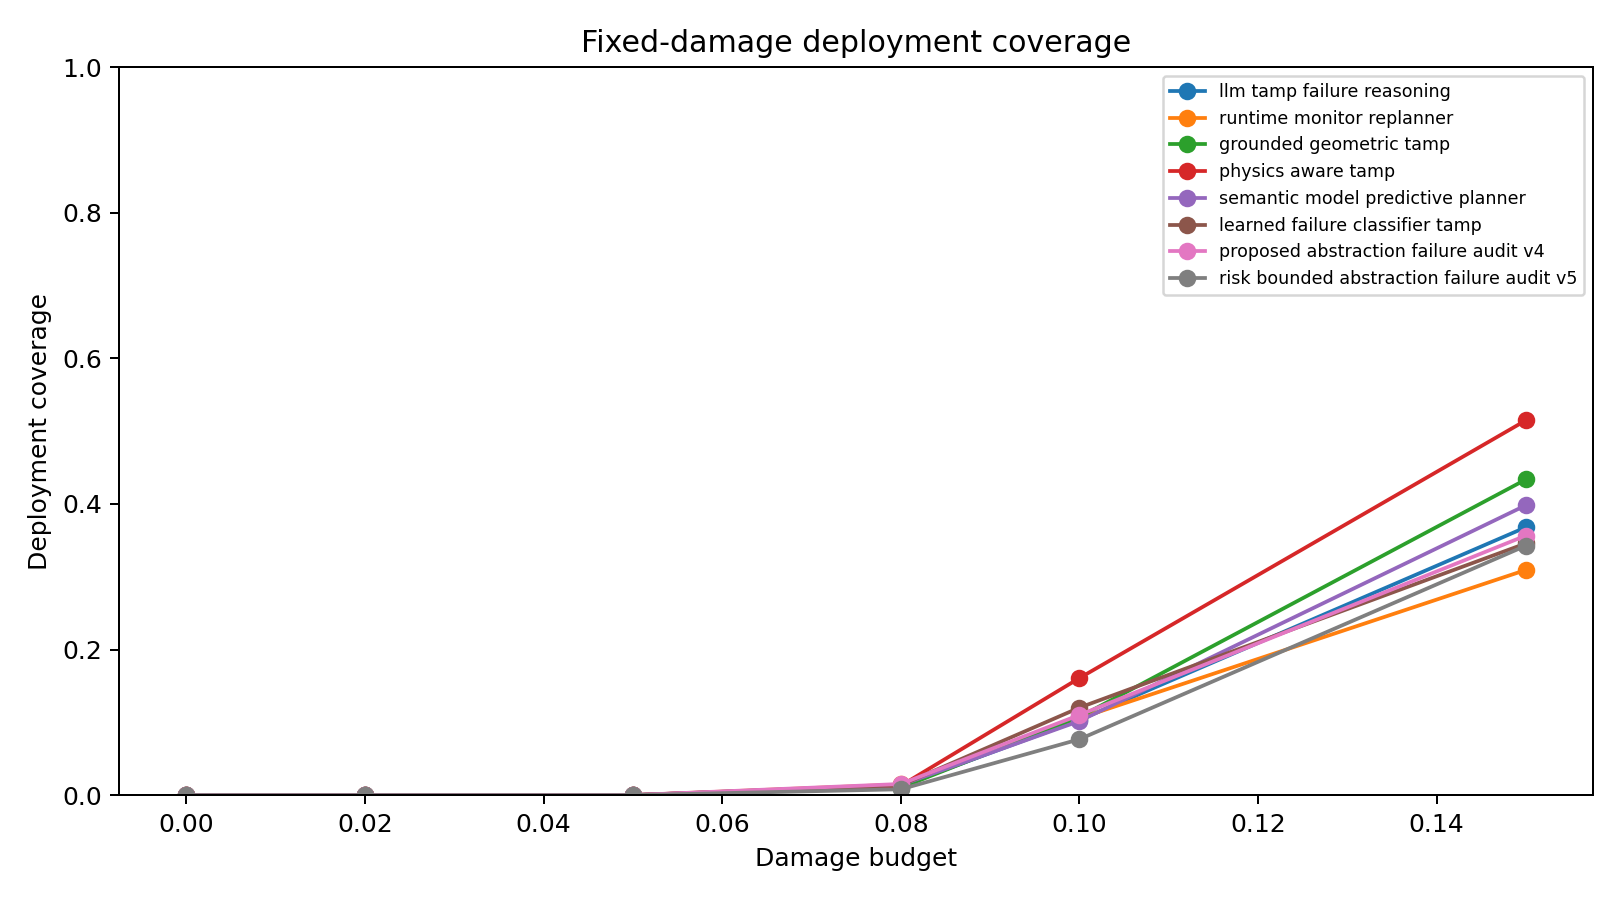
\includegraphics[width=0.88\linewidth]{abstraction_v5_fixed_risk.png}
\caption{Deployment coverage as the damage budget varies.}
\end{figure}

\section{Negative Cases}
The negative cases are selected by predefined high-regret, high-damage, high-violation, and low-success rules.

\begin{table}[H]
\centering
\caption{Representative failure cases.}
\label{tab:negative}
\resizebox{\linewidth}{!}{\begin{tabular}{lllllll}
\toprule
Split & Task & Failure & Success & Damage & Regret & Failure \\
\midrule
combined\_adversarial\_abstraction & tool\_use\_with\_hidden\_leverage & clearance\_tolerance\_collapse & 0.117088 & 0.431166 & 0.902022 & grounded or physics-aware TAMP captures the mechanics with lower regret \\
mechanics\_ood\_shift & container\_insertion\_clearance & clearance\_tolerance\_collapse & 0.122136 & 0.441373 & 0.898911 & grounded or physics-aware TAMP captures the mechanics with lower regret \\
combined\_adversarial\_abstraction & deformable\_object\_packing & clearance\_tolerance\_collapse & 0.120528 & 0.444209 & 0.896103 & grounded or physics-aware TAMP captures the mechanics with lower regret \\
combined\_adversarial\_abstraction & mobile\_manipulation\_with\_occlusion & clearance\_tolerance\_collapse & 0.133071 & 0.426199 & 0.881255 & grounded or physics-aware TAMP captures the mechanics with lower regret \\
combined\_adversarial\_abstraction & tool\_use\_with\_hidden\_leverage & clearance\_tolerance\_collapse & 0.141133 & 0.420436 & 0.871582 & grounded or physics-aware TAMP captures the mechanics with lower regret \\
mechanics\_ood\_shift & deformable\_object\_packing & clearance\_tolerance\_collapse & 0.155897 & 0.465825 & 0.871003 & grounded or physics-aware TAMP captures the mechanics with lower regret \\
combined\_adversarial\_abstraction & tool\_use\_with\_hidden\_leverage & deformable\_constraint\_erasure & 0.114090 & 0.491486 & 0.868293 & deformation risk remains high despite detecting the erased mechanics \\
combined\_adversarial\_abstraction & tabletop\_manipulation\_with\_support & clearance\_tolerance\_collapse & 0.146143 & 0.432156 & 0.867011 & grounded or physics-aware TAMP captures the mechanics with lower regret \\
\bottomrule
\end{tabular}
}
\end{table}

\section{Related Work Pressure}
The local literature pool is used as hostile pressure rather than as a claim that every record is directly applicable. VLA planning, neuro-symbolic predicates, relational abstraction, grounded TAMP, runtime monitoring, failure recovery, and deployment safety all pressure the novelty claim \citep{berahman2009probabilistic19,ying2025agentsafe20,jenamani2020robotic21} \citep{francis2022core22,huang2026neurosymbolic23,hayes2025finegrain24} \citep{capitanelli2024a25,chaudhary2026revealing26,agia2024unpacking27} \citep{kambhampati2023on28,johnson2023critical29,li2025survey30}.

The novelty boundary is narrow: an abstraction audit must beat grounded planning and failure reasoning on closed-loop deployment metrics, not just classify erased mechanics. The audit shows that it does not. Appendix~\ref{app:citations} provides clickable pressure chunks sourced from the shared pool.

\section{Limitations}
This is a local CPU-only executable audit. It is not real robot evidence, not an accepted high-fidelity simulator benchmark, not a trained checkpoint comparison, and not an external embodied-planning benchmark. The negative result falsifies the claim inside the frozen surrogate benchmark. A revival must gather external evidence and a stronger mechanism, not hide failed gates.

\section{Reproducibility}
Run \method{python src/run\_experiment.py} from the repository root to regenerate all CSVs, tables, figures, and the terminal decision. Then run \method{python scripts/generate\_manuscript.py} and compile \method{paper/main.tex} with pdflatex, BibTeX, and two more pdflatex passes. The final numbered PDF belongs only at \method{C:/Users/wangz/Downloads/99.pdf}.

\section{Conclusion}
Mechanics-aware abstraction audits are plausible, but this v5 evidence does not support a positive ICLR-main contribution. V5 avoids false refinements but collapses on success, violation, damage, regret, utility, ablation, stress, and fixed-risk gates. The honest decision is \textbf{KILL\_ARCHIVE}.

\clearpage
\appendix
\section{Full Gate Ledger}
\begin{longtable}{p{0.24\linewidth}p{0.66\linewidth}}
\toprule
Gate & Frozen outcome \\
\midrule
Success & Failed: v5 success 0.28708 trails physics\_tamp at 0.67262. \\
Violation & Failed: v5 violation 0.45954 trails physics\_tamp at 0.16450. \\
Damage & Failed: v5 damage 0.37043 trails physics\_tamp at 0.13935. \\
Regret & Failed: v5 regret 0.63814 trails physics\_tamp at 0.06982. \\
Utility & Failed: v5 utility -0.33399 trails physics\_tamp at 0.30626. \\
False alarm & Passed: v5 false alarm is 0.00026. \\
Ablation & Failed: all planned ablations match or beat full v5 on at least one predefined metric. \\
Stress & Failed: maximum stress is dominated by physics\_tamp. \\
Fixed risk & Failed: budget 0.05 is dominated by grounded\_tamp or insufficient coverage. \\
Scope & Failed: no hardware, accepted high-fidelity benchmark, external benchmark, or trained checkpoint evidence. \\
\bottomrule
\end{longtable}

\section{Metric Definitions}
Task success is expected closed-loop completion. Mechanical violation is action-incompatible contact, support, clearance, friction, deformation, or tool-use violation. Damage is expected unsafe action or object/fixture damage. Abstraction-failure accuracy measures hidden mechanics-erasure classification. Mechanics-retention recall measures whether the action preserves relevant mechanics on actionable failures. False alarm is heavy intervention on temporal or nuisance cases. Robust utility subtracts violation, damage, cost, and abstention penalties from success. Regret is the gap to a non-deployable oracle action.

\section{Expanded Baseline Descriptions}
Language symbolic planning trusts high-level predicates. VLA direct policy maps observations and language to actions. Neuro-symbolic predicates learn abstract state tests. Active relational abstraction asks for predicate grounding. LLM-TAMP failure reasoning routes failures through task-and-motion planning. Runtime monitoring replans after risk appears. Grounded geometric TAMP exposes geometry directly. Physics-aware TAMP exposes geometry and mechanics. Affordance graphs reason over object-use relations. Learned failure classifier plus TAMP uses a classifier before planning. Semantic MPC plans over symbolic and continuous risk features. V4 and v5 test the proposed abstraction-failure audit.

\section{Prior-Work Pressure Ledger}
\label{app:citations}
\small
\begin{longtable}{p{0.06\linewidth}p{0.38\linewidth}p{0.48\linewidth}}
\toprule
ID & Pressure role & Clickable citations \\
\midrule
1 & VLA and language abstraction pressure & \citep{li2023embodied1,liang2024visualpredicator2,devinda3} \\
2 & neuro-symbolic predicate pressure & \citep{farid2026vision4,ahn2025towards5,park2025hierarchical6} \\
3 & relational abstraction and active learning pressure & \citep{pang2025integrating7,shao2025breaking8,wu2023embodied9} \\
4 & task-and-motion planning pressure & \citep{shao2024breaking10,chen2026oowm11,liu2026bioproagent12} \\
5 & monitoring, recovery, and failure reasoning pressure & \citep{virwani2025loop13,yang2023weizenbaums14,pallagani2024on15} \\
6 & safety, deployment, and reproducibility pressure & \citep{vinay2026a16,wang2024llm17,mooneeram2013literary18} \\
7 & VLA and language abstraction pressure & \citep{berahman2009probabilistic19,ying2025agentsafe20,jenamani2020robotic21} \\
8 & neuro-symbolic predicate pressure & \citep{francis2022core22,huang2026neurosymbolic23,hayes2025finegrain24} \\
9 & relational abstraction and active learning pressure & \citep{capitanelli2024a25,chaudhary2026revealing26,agia2024unpacking27} \\
10 & task-and-motion planning pressure & \citep{kambhampati2023on28,johnson2023critical29,li2025survey30} \\
11 & monitoring, recovery, and failure reasoning pressure & \citep{andreyev2026bounding31,chen2026from32,zhu2025psalmv33} \\
12 & safety, deployment, and reproducibility pressure & \citep{dawson2023a34,basir2022critical35,diwakaruni2026ai36} \\
13 & VLA and language abstraction pressure & \citep{vegabrown2018admissible37,deng2025automating38,chatterjeendinferencetime39} \\
14 & neuro-symbolic predicate pressure & \citep{olaiya2025from40,kong2025embodied41,liu2012planning42} \\
15 & relational abstraction and active learning pressure & \citep{chen2024languageaugmented43,dogangun2026bilevel44,mizoguchi2022abstractionbased45} \\
16 & task-and-motion planning pressure & \citep{coluzzi2017language46,hemken2023how47,shah2024learning48} \\
17 & monitoring, recovery, and failure reasoning pressure & \citep{kwon2025fast49,shirai2023visionlanguage50,kwon2024fast51} \\
18 & safety, deployment, and reproducibility pressure & \citep{tosello2026interleaving52,johnson2018research53,wachter2018integrating54} \\
19 & VLA and language abstraction pressure & \citep{huang2022inner55,francis2023core56,kostin2025padlabeling57} \\
20 & neuro-symbolic predicate pressure & \citep{jia2024langsuite58,yu2025mowm59,li2026worldvalueaction60} \\
21 & relational abstraction and active learning pressure & \citep{liu2026agentic61,chen2025codeassymbolicplanner62,lorang2026build63} \\
22 & task-and-motion planning pressure & \citep{yang2026nesyroute64,din2025lang2manip65,zhai2026cascading66} \\
23 & monitoring, recovery, and failure reasoning pressure & \citep{yevdokymov2024neurosymbolic67,cai2024neusis68,ref2026multimodal69} \\
24 & safety, deployment, and reproducibility pressure & \citep{jung2020software70,hwang2025how71,wang2025where72} \\
25 & VLA and language abstraction pressure & \citep{shah2023reliable73,he2024utilizing74,skerrett2016moving75} \\
26 & neuro-symbolic predicate pressure & \citep{sunndfrontiers76,suriani2026modeling77,slaouindsairobotics78} \\
27 & relational abstraction and active learning pressure & \citep{ali2026neurosymbolic79,p2025proactive80,slaoui2026sairobotics81} \\
28 & task-and-motion planning pressure & \citep{silver2022learning82,song2025rcienhanced83,hu2025reinforcement84} \\
29 & monitoring, recovery, and failure reasoning pressure & \citep{chen2025multimodal85,lan2025active86,niu2025research87} \\
30 & safety, deployment, and reproducibility pressure & \citep{byrd2026constrained88,son2026software89,moncadaramirez2025agentic90} \\
31 & VLA and language abstraction pressure & \citep{zhang2025mitigating91,galitsky2026neurosymbolic92,berg2022using93} \\
32 & neuro-symbolic predicate pressure & \citep{chalvatzaki2023learning94,maclean2021where95,zhou2024isrllm96} \\
33 & relational abstraction and active learning pressure & \citep{mitterer2024automating97,skerrett2014the98,han2025development99} \\
34 & task-and-motion planning pressure & \citep{winter2006trajectories100,zhang2024badrobot101,zenil2026on102} \\
35 & monitoring, recovery, and failure reasoning pressure & \citep{wangndbridging103,shirai2024visionlanguage104,wang2024large105} \\
36 & safety, deployment, and reproducibility pressure & \citep{liang2023code106,dobrovsky2025intelligent107,hsu2025from108} \\
37 & VLA and language abstraction pressure & \citep{dearden2014manipulation109,fu2022the110,yang2025guiding111} \\
38 & neuro-symbolic predicate pressure & \citep{xie2024embodiedrag112,park2023deep113,buehler2024xlora114} \\
39 & relational abstraction and active learning pressure & \citep{hamilton2024is115,wu2025a116,quan2020critical117} \\
40 & task-and-motion planning pressure & \citep{tsushima2025task118,dai2024optimal119,yang2025planllm120} \\
41 & monitoring, recovery, and failure reasoning pressure & \citep{chen2025affordancesoriented121,torralba2018symbolic122,ref2018the123} \\
42 & safety, deployment, and reproducibility pressure & \citep{sakib2025star124,pacaud2025scaling125,lynch1996stable126} \\
43 & VLA and language abstraction pressure & \citep{zhou2026opendrivevla127,wang2025conformal128,yi2024applications129} \\
44 & neuro-symbolic predicate pressure & \citep{wang2025probabilistically130,konidaris2018from131,yu2025mutpllm132} \\
45 & relational abstraction and active learning pressure & \citep{shi2025scvlm133,joseph2023large134,yuendplanagent135} \\
46 & task-and-motion planning pressure & \citep{sakib2025star136,yang2024adapt2reward137,fu2024degradation138} \\
47 & monitoring, recovery, and failure reasoning pressure & \citep{li2026tcot139,rubavicius2025learning140,matthewmanndlarge141} \\
48 & safety, deployment, and reproducibility pressure & \citep{suvarna2023language142,vlaeva2021vision143,hao2023reasoning144} \\
49 & VLA and language abstraction pressure & \citep{zhang2025llmgrop145,hutahaean2025use146,perezmilans2018language147} \\
50 & neuro-symbolic predicate pressure & \citep{mohammadi2026parameterefficient148,liu2026arassisted149,winter2008trajectories150} \\
51 & relational abstraction and active learning pressure & \citep{baxter2023interpreting151,lyu2019sdrl152,schakkal2025hierarchical153} \\
52 & task-and-motion planning pressure & \citep{ding2026unilavira154,mu2024pix2planning155,kobilov2025automatic156} \\
53 & monitoring, recovery, and failure reasoning pressure & \citep{chu2025llmmap157,colan2025assessing158,lafon2025vilu159} \\
54 & safety, deployment, and reproducibility pressure & \citep{chen2026reconvla160,gu2025safe161,yang2025fpcvla162} \\
55 & VLA and language abstraction pressure & \citep{stewart2023large163,zhang2024firerobbrain164,ma2026a165} \\
56 & neuro-symbolic predicate pressure & \citep{liu2019languagelike166,zhou2024hard167,wang2024large168} \\
57 & relational abstraction and active learning pressure & \citep{hoffman2025feasibility169,yuxian2025bridging170,huang2025planning171} \\
58 & task-and-motion planning pressure & \citep{matuszek2021grounded172,aryashad2025vlag173,aghzal2024evaluating174} \\
59 & monitoring, recovery, and failure reasoning pressure & \citep{ordem2023participatory175,liu2026from176,wang2025image177} \\
60 & safety, deployment, and reproducibility pressure & \citep{green2022motion178,liu2026task179,lozano2025invisible180} \\
61 & VLA and language abstraction pressure & \citep{chen2026sustainable181,lin2024clmasp182,zhu2026designing183} \\
62 & neuro-symbolic predicate pressure & \citep{belta2005discrete184,silva2024robotic185,ganai2025realtime186} \\
63 & relational abstraction and active learning pressure & \citep{chen2025codeassymbolicplanner187,lu2025probing188,kwon2025large189} \\
64 & task-and-motion planning pressure & \citep{burbridge2012learning190,shankar2024abstract191,boer2025design192} \\
65 & monitoring, recovery, and failure reasoning pressure & \citep{rana2023sayplan193,yoshikawa2023developing194,joublin2023copal195} \\
66 & safety, deployment, and reproducibility pressure & \citep{hunttaliilaogwa2024against196,hong2024multiply197,du2023video198} \\
67 & VLA and language abstraction pressure & \citep{xie2023languageconditioned199,yang2023on200,kannan2023smartllm201} \\
68 & neuro-symbolic predicate pressure & \citep{xie2023translating202,lee2023systemlevel203,zhang2025embodied204} \\
69 & relational abstraction and active learning pressure & \citep{liu2025investigation205,lorangndbuild206,fan2026navla2207} \\
70 & task-and-motion planning pressure & \citep{dhole2025aipowered208,shah2022using209,zhou2025rt2210} \\
71 & monitoring, recovery, and failure reasoning pressure & \citep{sun2026dadue211,tang2026sltp212,du2023video213} \\
72 & safety, deployment, and reproducibility pressure & \citep{feng2024task214,kumar2026openworld215,kobilov2025automatic216} \\
73 & VLA and language abstraction pressure & \citep{boya2025large217,certo2025large218,bonda2025hoverbvi219} \\
74 & neuro-symbolic predicate pressure & \citep{han2025traffic220,halacheva2025gaussianvlm221,choi2025find222} \\
75 & relational abstraction and active learning pressure & \citep{singh2025llmrspf223,paradowskindthe224,murata2026multirobot225} \\
76 & task-and-motion planning pressure & \citep{li2025from226,sun2025llapa227,kantaros2020reactive228} \\
77 & monitoring, recovery, and failure reasoning pressure & \citep{mcenteeatalianis2016a229,bamgbo2003a230} \\
\bottomrule
\end{longtable}

\bibliographystyle{plainnat}
\bibliography{references}
\end{document}
